\section{Opis interfejsu}

\begin{figure}[!h]
	\center
	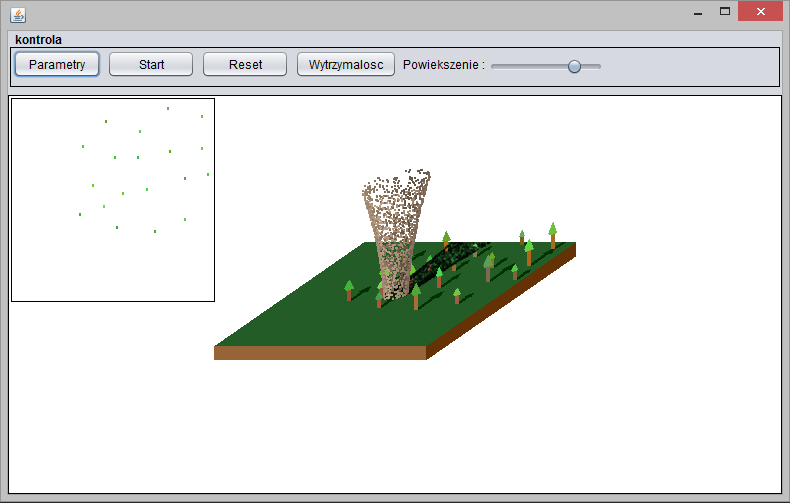
\includegraphics[scale=0.75]{gui_main}
	\caption{Główne okno programu.}
	\label{fig:gui_main}
\end{figure} 

Uruchamienie aplikacji symulacji powoduje wyświetlenie głównego okna programu (Rysunek~\ref{fig:gui_main}). W centralnej ramce ukazana jest wizualizacja zjawiska w rzucie izometrycznym. Ukazuje ona symboliczną strukturę lasu i położenie tornada. Drzewa nieuszkodzone mają pień koloru brązowego oraz zieloną koronę, drzewa złamane wizualizowane są w kolorze czerwonym, a drzewa przewrócone w kolorze niebieskim. W lewym górnym rogu ukazany jest rzut lasu z góry, który posiada taką samą konwencję kolorów jak wizualizacja 3D. Można na nim dokładniej zaobserwować kierunki działania wiatru tornada przy przewracaniu drzew.

Dodatkowo, przytrzymując przycisk \textbf{Wytrzymałość} możliwa jest wizualizacja potencjalnej wytrzymałości drzew wyliczana na podstawie otoczenia każdego z nich. Kolor niebieski oznacza najmniej wytrzymałe drzewo, czyli znajdujące się na skraju lasu i/lub nieposiadające bliskich sąsiadów. Im korona bardziej przechodzi w kolor czerwony, drzewo klasyfikowane jest jako bardziej wytrzymałe dzięki tłumieniu wiatru przez drzewa położone w najbliższym jego otoczeniu.

 Nad ramką wizualizacji znajduje się panel sterowania symulacją. Dotępne przyciski kontroli to:

\begin{itemize}
\item \textbf{Parametry} -- wyświetlenie okna ustawiania parametrów symulacji oraz właściwości modeli Rankine i HWind.
\item \textbf{Start/Stop} -- rozpoczęcie/zatrzymanie symulacji.
\item \textbf{Reset} -- przywrócenie wartości początkowych (ustawionych w oknie Parametry) symulacji, wygenerowanie nowego lasu.
\item \textbf{Wytrzymałość} -- przytrzymanie tego przycisku powoduje wyświetlenie informacji o wytrzymałości drzew w postaci kolorów.
\end{itemize}

Ponadto, istnieje możliwość zmiany skali wizualizacji przesuwając suwak z etykietą ,,Powiększenie'' na pożadaną pozycję.



\subsection{Okno parametrów symulacji}

Wygląd interfejsu manipulacji parametrami programu przedstawia rysunek~\ref{fig:gui_param}.

W ramce \textbf{Świat} możemy ustawić wymiary (szerokość i długość) siatki, na której zostanie wygenerowany las.

Ramka \textbf{Wir} pozwala na manipulację parametrami modelu wiru Rankine. Posiada następujące kontrolki:
\begin{itemize}
\item
\end{itemize}

\begin{figure}[!h]
	\center
	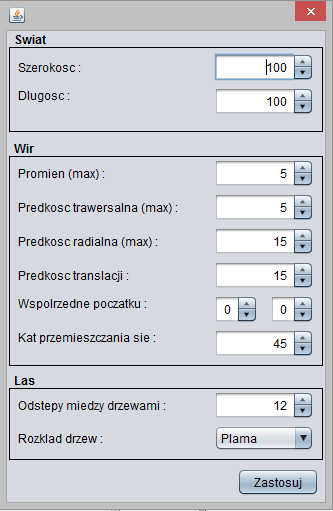
\includegraphics[scale=1]{gui_param}
	\caption{Okno ustawiania parametrów symulacji.}
	\label{fig:gui_param}
\end{figure} 